\documentclass{beamer}
\usepackage[utf8]{inputenc}
\usepackage{amsmath}
\usepackage{amsfonts}
\usepackage{amssymb}
\usepackage{makeidx}
\usepackage{graphicx}
\usepackage{lmodern}
\usepackage{color}
\usepackage{xcolor}
\usepackage{bussproofs}
\usepackage{lscape}
\usepackage{listings}
\usepackage{amsthm}
\usetheme{CambridgeUS}

\usefonttheme{serif}

\title{Type checker for system F}
\author{Mudathir Mahgoub}
  
 
\begin{document}
 
\frame{\titlepage}
 
\begin{frame}
\frametitle{Type checking problem}

Given a typing context $\Gamma$ and  a term $t$ and a type $T$, can the term $t$ be assigned the type $T$ under the typing context $\Gamma$?

Is the judgment $\Gamma \vdash t: T$  derivable?
\end{frame}

\begin{frame}
\frametitle{Software components}
\begin{figure}
 \centering
 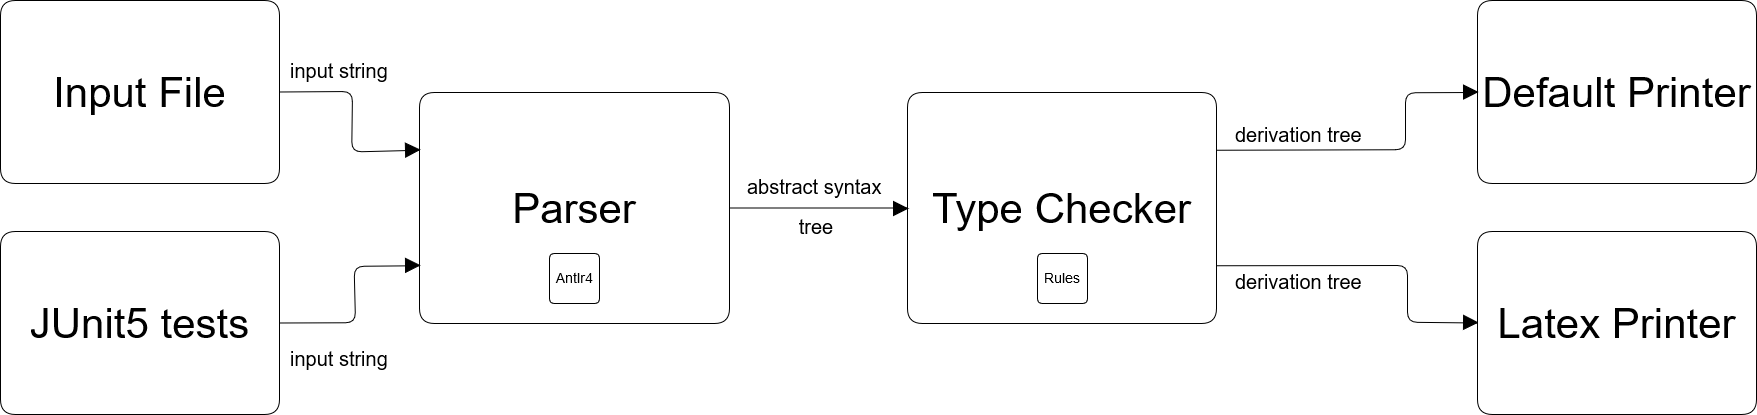
\includegraphics[scale=.18,keepaspectratio=true]{./typechecker.png}
\end{figure}
\end{frame}

%\definecolor{light-gray}{gray}{0.95}
%\lstset{backgroundcolor= \color{light-gray}} 

\begin{frame}[fragile]
\frametitle{Execution}
\scriptsize

\begin{block}{Input: test.txt}
\begin{lstlisting}  
SubBase(bool, int);
. |- \lambda x. \lambda y. (x y)[bool]: (int ->T) -> (bool -> T);
\end{lstlisting}
\end{block}

\begin{block} {Output: java -jar TypeChecker.jar -i test.txt}
\begin{lstlisting}
Yes  
                        	SubBase(bool, int)	
-------------------(var)	-------------------(subBase)	
x: bool |- x : bool			bool <: int
--------------------------------------(subsumption)
x: bool |- x : int
\end{lstlisting}
\end{block}

\end{frame} 


\begin{frame}[fragile]
\frametitle{Execution}
\scriptsize

\begin{block}{Input: test.txt}
\begin{lstlisting}  
SubBase(bool, int);
. |- \lambda x. \lambda y. (x y)[bool]: (int ->T) -> (bool -> T);
\end{lstlisting}
\end{block}

\begin{block} {Output: java -jar TypeChecker.jar -i test.txt -latex}
\begin{lstlisting}  
Yes
\begin{prooftree}
\AxiomC{} 
\RightLabel{\scriptsize var}
\UnaryInfC{$x: bool \vdash x : bool$}
\AxiomC{\scriptsize $SubBase(bool,int)$}
\RightLabel{\scriptsize subBase}
\UnaryInfC{$bool <: int$}
\RightLabel{\scriptsize subsumption}
\BinaryInfC{$x: bool \vdash x : int$}
\end{prooftree}
\end{lstlisting}
\end{block}
\end{frame} 

\begin{frame} 
\frametitle{Demo}
\begin{block}{Demo}
\end{block}
\end{frame} 

\begin{frame} 
\frametitle{Simple types}
\begin{block}{Terms}
\begin{align*}
t::= x \;|\; (t_1 t_2)\color{blue}[T]\color{black}\;|\; \lambda x.t
\end{align*}
\end{block}

\begin{block}{Typing rules}
\begin{enumerate}

\item Variable rule
\begin{prooftree}
\AxiomC{$\Gamma (x) = T$} \RightLabel{\scriptsize var} \UnaryInfC{$\Gamma \vdash x : T$}
\end{prooftree}
\item Application rule
\begin{prooftree}
\AxiomC{$\Gamma \vdash t_1 : T_1 \rightarrow T_2$} 
\AxiomC{$\Gamma \vdash t_2 : T_1$}
 \RightLabel{\scriptsize app} \BinaryInfC{$\Gamma \vdash (t_1 t_2)\color{blue}[T_1] \color{black} : T_2$}
\end{prooftree}
\item $\lambda$ rule
\begin{prooftree}
\AxiomC{$\Gamma, x:T_1 \vdash t : T_2$} 
 \RightLabel{\scriptsize $\lambda$} \UnaryInfC{$\Gamma \vdash \lambda x .t:  T_1 \rightarrow T_2$}
\end{prooftree}

\end{enumerate}
\end{block}
\end{frame} 


\begin{frame} 
\frametitle{Simple types}
\begin{block}{Subtyping rules}


\begin{prooftree}
\AxiomC{$\Gamma \vdash t : T_1$} 
\AxiomC{$T_1 <: T_2$}
 \RightLabel{\scriptsize subsumption} \BinaryInfC{$\Gamma \vdash t: T_2$}
\end{prooftree}


\begin{prooftree}
\AxiomC{} 
 \RightLabel{\scriptsize reflexive} \UnaryInfC{$T <: T$}
\end{prooftree}


\begin{prooftree}
\AxiomC{$SubBase(b_1, b_2)$} 
 \RightLabel{\scriptsize subBase} \UnaryInfC{$b_1 <: b_2$}
\end{prooftree}


\begin{prooftree}
\AxiomC{$T'_1 <: T_1$} 
\AxiomC{$T_2 <: T'_2$}
 \RightLabel{\scriptsize arrow} \BinaryInfC{$T_1 \rightarrow T_2 <: T'_1 \rightarrow T'_2$}
\end{prooftree}



\begin{prooftree}
\AxiomC{$T_1 <: T_2$} 
\AxiomC{$T_2 <: T_3$}
 \RightLabel{\scriptsize transitive} \BinaryInfC{$T_1 <: T_3$}
\end{prooftree}
\end{block}
\end{frame} 
 
\begin{frame}
\frametitle{Simple types}
\begin{block} {Examples}
\begin{prooftree}
\AxiomC{} \RightLabel{\scriptsize var} \UnaryInfC{$x: T \vdash x : T$}
\end{prooftree}

\begin{prooftree}
\AxiomC{} \RightLabel{\color{red} \scriptsize invalid var} \UnaryInfC{$\cdot \vdash x : T$} \color{black} 
\end{prooftree}

\scriptsize

\begin{prooftree}
\AxiomC{} \RightLabel{var} \UnaryInfC{$x: (T_1 \rightarrow T_2), y: T_1 \vdash x : (T_1 \rightarrow T_2)$}
\AxiomC{} \RightLabel{var} \UnaryInfC{$x: (T_1 \rightarrow T_2), y: T_1 \vdash y : T_1$}
\RightLabel{app} \BinaryInfC{$x: (T_1 \rightarrow T_2), y: T_1 \vdash (x\;y) [T_1] : T_2$}
\RightLabel{$\lambda$}\UnaryInfC{$x: (T_1 \rightarrow T_2) \vdash  \lambda y. (x\;y) [T_1] : (T_1 \rightarrow T_2)$}
\RightLabel{$\lambda$}\UnaryInfC{$\cdot \vdash  \lambda x.  \lambda y. (x\;y) [T_1] : ((T_1 \rightarrow T_2) \rightarrow (T_1 \rightarrow T_2))$}
\end{prooftree}

\end{block}
\end{frame} 


\begin{frame}
\frametitle{Subtyping}
\begin{block} {Examples}

\begin{prooftree}
\AxiomC{} \RightLabel{\scriptsize var} \UnaryInfC{$x: bool \vdash x : bool$}
\AxiomC{\scriptsize SubBase($bool,int)$} \RightLabel{\scriptsize subBase} \UnaryInfC{$bool <: int$}
\RightLabel{\scriptsize subsumption} \BinaryInfC{$x: bool \vdash x : int$}
\end{prooftree}

\begin{prooftree}
\AxiomC{} \RightLabel{\scriptsize var} \UnaryInfC{$x: int \vdash x : int$}
\AxiomC{\color{red} $\perp$ \color{black}} \RightLabel{\scriptsize \color{red} invalid \color{black}} \UnaryInfC{\color{red} $int <: bool$ \color{black}}
\RightLabel{\scriptsize subsumption} \BinaryInfC{$x: int \vdash x : bool$}
\end{prooftree}

\scriptsize
\begin{prooftree}
\AxiomC{} \RightLabel{\scriptsize var} \UnaryInfC{$x: bool \vdash x : bool$}
\AxiomC{\scriptsize SubBase($bool,int)$} \RightLabel{\scriptsize subBase} \UnaryInfC{$bool <: int$}
\AxiomC{\scriptsize SubBase($int,double)$} \RightLabel{\scriptsize subBase} \UnaryInfC{$int <: double$}
\RightLabel{\scriptsize transitive} \BinaryInfC{$bool <: double$}
\RightLabel{\scriptsize subsumption} \BinaryInfC{$x: bool \vdash x : double$}
\end{prooftree}

\end{block}
\end{frame}

\color{black}
\begin{frame}
\frametitle{Subtyping}
\begin{figure}
 \centering
 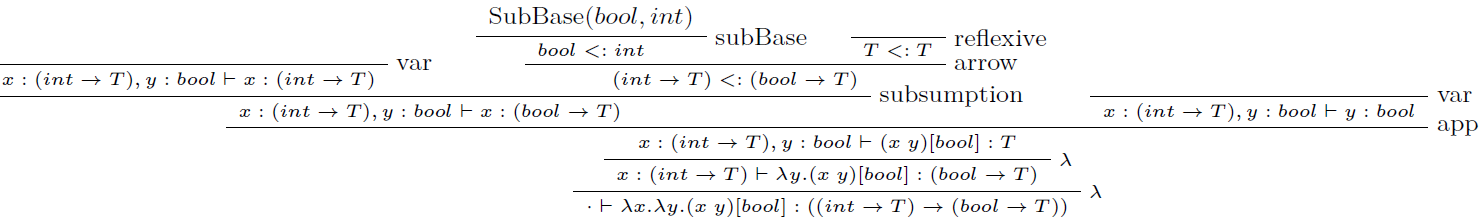
\includegraphics[scale=.30,keepaspectratio=true]{./subsumption.png}
\end{figure}
\end{frame}

\begin{frame}
\frametitle{Delaying the subsumption rule}
\begin{block}{Remark}
The sumbumption rule can be delayed until the term in the judgment is a variable.
\end{block}

\begin{prooftree}
\AxiomC{$\Gamma \vdash t : T$} 
\AxiomC{$T <: T'$}
 \RightLabel{\scriptsize subsumption} \BinaryInfC{$\Gamma \vdash t: T'$}
\end{prooftree}
\end{frame}

\begin{frame}
\frametitle{Delaying the subsumption rule}
Case $t=x$: trivial since $t$ is a variable. 

\begin{prooftree}
\AxiomC{$\Gamma \vdash x : T$} 
\AxiomC{$T <: T'$}
 \RightLabel{\scriptsize subsumption} \BinaryInfC{$\Gamma \vdash x: T'$}
\end{prooftree}
\end{frame}


\begin{frame}
\frametitle{Delaying the subsumption rule}
Case $t=t_1 t_2$: assume $T_2 <: T'_2$ and the following derivation:

\begin{prooftree}
\AxiomC{\color{blue} $\Gamma \vdash t_1 : T_1 \rightarrow T_2$ \color{black}} 
\AxiomC{\color{blue} $\Gamma \vdash t_2 : T_1$ \color{black}} 
\RightLabel{\scriptsize app}
\BinaryInfC{$\Gamma \vdash (t_1 t_2) [T_1] : T_2$} 
\AxiomC{\color{blue} $T_2 <: T'_2$ \color{black}}
\RightLabel{\scriptsize subsumption} 
\BinaryInfC{$\Gamma \vdash (t_1 t_2) [T_1]: T_2'$}
\end{prooftree}

Alternatively

\scriptsize
\begin{prooftree}
\AxiomC{\color{blue} $\Gamma \vdash t_1 : T_1 \rightarrow T_2$ \color{black}} 
\AxiomC{} 
\RightLabel{\scriptsize reflexive}
\UnaryInfC{$T_1 <: T_1$} 
\AxiomC{\color{blue} $T_2 <: T'_2$ \color{black}}
\RightLabel{\scriptsize arrow}
\BinaryInfC{$T_1 \rightarrow T_2 <: T_1 \rightarrow T'_2$}
\RightLabel{\scriptsize subsumption}
\BinaryInfC{$\Gamma \vdash t_1 : T_1 \rightarrow T'_2$} 
\AxiomC{\color{blue} $\Gamma \vdash t_2 : T_1$ \color{black}} 
\RightLabel{\scriptsize app} 
\BinaryInfC{$\Gamma \vdash (t_1 t_2) [T_1]: T'_2$}
\end{prooftree}

\end{frame}


\begin{frame}
\frametitle{Delaying the subsumption rule}
Case $t=\lambda x. t'$: assume $T_1 \rightarrow T_2 <: T'_1 \rightarrow T'_2$ and the following derivation:

\begin{prooftree}
\AxiomC{\color{blue} $\Gamma, x:  T_1 \vdash t': T_2$ \color{black}} 
\RightLabel{\scriptsize $\lambda$}
\UnaryInfC{$\Gamma \vdash \lambda x. t': T_1 \rightarrow T_2$} 
\AxiomC{\color{blue} $T'_1 <: T_1$ \color{black}} 
\AxiomC{\color{blue} $T_2 <: T'_2$ \color{black}}
\RightLabel{\scriptsize arrow} 
\BinaryInfC{$T_1 \rightarrow T_2 <: T'_1 \rightarrow T'_2$}
\RightLabel{\scriptsize subsumption} 
\BinaryInfC{$\Gamma \vdash \lambda x. t': T'_1 \rightarrow T'_2$}
\end{prooftree}

Alternatively

\begin{prooftree}
\AxiomC{\color{blue} $\Gamma, x: T'_1  \vdash t':  T_2$ \color{black}} 
\AxiomC{\color{blue} $T_2 <: T'_2$ \color{black}}
\RightLabel{\scriptsize subsumption} 
\BinaryInfC{$\Gamma, x: T'_1  \vdash t':  T'_2$} 
\RightLabel{\scriptsize $\lambda$} 
\UnaryInfC{$\Gamma \vdash \lambda x. t': T'_1 \rightarrow T'_2$}
\end{prooftree}

Assuming \color{blue} $T'_1 <: T_1$ \color{black} is derivable, then by the subsumption rule:
\begin{prooftree}
\AxiomC{}
\RightLabel{\scriptsize var} 
\UnaryInfC{$\Gamma, x: T'_1 \vdash  x : T'_1 $}
\AxiomC{\color{blue} $T'_1 <: T_1$ \color{black}}
\RightLabel{\scriptsize subsumption} 
\BinaryInfC{$\Gamma, x: T'_1 \vdash \color{blue} x : T_1 \color{black} $}
\end{prooftree}

\end{frame}


\begin{frame}
\frametitle{Delaying the subsumption rule}
\begin{block} {Remark}
If $T'_1 <: T_1$ and $\Gamma, x: T'_1  \vdash t':  T_2$, it is not always true  that $\Gamma, x: T_1  \vdash t':  T_2$.
\end{block}

\begin{block} {Counter example}
\begin{align*}
x: bool \vdash x: int \nRightarrow x:double \vdash x: int,\;\;\; bool <: int <: double
\end{align*}
\end{block}

\begin{block} {}
\begin{align*}
x: int \vdash x: double \Rightarrow x:bool \vdash x: double,\;\;\; bool <: int <: double
\end{align*}
\end{block}

\end{frame}


\begin{frame}

\scriptsize

\frametitle{Delaying the subsumption rule}
\begin{prooftree}
\AxiomC{\color{red} $\ x:  double \vdash x: int$ \color{black}} 
\RightLabel{\scriptsize $\lambda$}
\UnaryInfC{$\Gamma \vdash \lambda x. x: double \rightarrow int$} 
\AxiomC{$SubBase(bool, double)$}
\RightLabel{\scriptsize subBase} 
\UnaryInfC{$bool <: double$} 
\AxiomC{}
\RightLabel{\scriptsize reflexive} 
\UnaryInfC{$int <: int$}
\RightLabel{\scriptsize arrow} 
\BinaryInfC{$double \rightarrow int <: bool \rightarrow int$}
\RightLabel{\scriptsize subsumption} 
\BinaryInfC{$\Gamma \vdash \lambda x. x: bool \rightarrow int$}
\end{prooftree}

\normalsize
\begin{prooftree}
\AxiomC{} 
\RightLabel{\scriptsize var} 
\UnaryInfC{$\Gamma, x: bool \vdash x:  bool$} 
\AxiomC{$SubBase(bool, int)$} 
\RightLabel{\scriptsize subBase} 
\UnaryInfC{$bool <: int$}
\RightLabel{\scriptsize subsumption} 
\BinaryInfC{$\Gamma, x: bool  \vdash x:  int$} 
\RightLabel{\scriptsize $\lambda$} 
\UnaryInfC{$\Gamma \vdash \lambda x. x: bool \rightarrow int$}
\end{prooftree}

\end{frame}

\begin{frame}
\frametitle{System F}
\begin{block}{Terms}
\begin{align*}
t &::= x \;|\; (t_1 t_2)\color{blue}[T]\color{black}\;|\; \lambda x.t\; | \; t\; \color{blue} [[T]] \color{black}
\end{align*}
\end{block}

\begin{block}{Types}
\begin{align*}
T &::= X \; | T_1 \rightarrow T_2 \; | \; \forall X. T
\end{align*}
\end{block}

\end{frame}

\begin{frame}
\frametitle{System F additional rules}
\begin{enumerate}

\item If $X$ is not free in $\Gamma$

\begin{prooftree}
\AxiomC{$\Gamma \vdash t: T$} 
\RightLabel{\scriptsize introduction} 
\UnaryInfC{$\Gamma \vdash t: \forall X.T$}
\end{prooftree}

\item If $X$ is free in $\Gamma$, choose $X_i$ such that $X_i$ is not free in $\Gamma$

\begin{prooftree}
\AxiomC{$\Gamma \vdash t: [X_i/X]T$} 
\RightLabel{\scriptsize introduction} 
\UnaryInfC{$\Gamma \vdash t: \forall X_i.[X_i/X]T$} 
\RightLabel{\scriptsize renaming} 
\UnaryInfC{$\Gamma \vdash t: \forall X.T$}
\end{prooftree}

\item Elimination rule with annotation

\begin{prooftree}
\AxiomC{$\Gamma \vdash t: \forall X. \; \color{blue} [X/T']T \color{black}$} 
\RightLabel{\scriptsize elimination} 
\UnaryInfC{$\Gamma \vdash t\;\color{blue}[[T']]\color{black}: T$}
\end{prooftree}

\end{enumerate}

\end{frame}

\begin{frame}
\frametitle{System F examples}

\begin{itemize}

\item Different variables
\begin{prooftree}
\AxiomC{} \RightLabel{\scriptsize var} \UnaryInfC{$x: \forall X.(X \rightarrow X) \vdash x : \forall Y.(Y \rightarrow Y)$}
\end{prooftree}

\item $Y$ is free in the typing context and the term type

\begin{prooftree}
\AxiomC{} \RightLabel{\scriptsize var} \UnaryInfC{$x: \forall X.(X \rightarrow Y) \vdash x : \forall Z.(Z \rightarrow Y)$}
\end{prooftree}

\item $Y$ is free in the typing context
\begin{prooftree}
\AxiomC{} \RightLabel{\color{red} \scriptsize invalid var} \UnaryInfC{$x: \forall X.(X \rightarrow Y) \vdash x : \forall Y.(Y \rightarrow Y)$} \color{black} 
\end{prooftree}

\item $Y$ is free in the typing context, and $Z$ is free in the term type

\begin{prooftree}
\AxiomC{} \RightLabel{\color{red} \scriptsize invalid var} \UnaryInfC{$x: \forall X.(X \rightarrow Y) \vdash x : \forall Y.(Y \rightarrow Z)$} \color{black} 
\end{prooftree}

\end{itemize}
\end{frame}

\begin{frame}
\frametitle{System F examples}

\begin{itemize}

\item Elimination annotation
\begin{prooftree}
\AxiomC{} \RightLabel{\scriptsize var} \UnaryInfC{$x: \forall X.X \vdash x : \forall X1.\; \color{blue} X1$ \color{black}}
\RightLabel{\scriptsize elimination}\UnaryInfC{$x: \forall X.X \vdash x \color{blue}[[Y]] \color{black} : Y$}
\end{prooftree}

\item Elimination annotation with arrow
\begin{prooftree}
\AxiomC{} \RightLabel{\scriptsize var} \UnaryInfC{$x: \forall X.X \vdash x : \forall X1. \; \color{blue}X1\color{black}$ }
\RightLabel{\scriptsize elimination}\UnaryInfC{$x: \forall X.X \vdash  x\color{blue}[[(Y \rightarrow Y)]] \color{black} : (Y \rightarrow Y)$}
\end{prooftree}
\end{itemize}
\end{frame}

\begin{frame}
\frametitle{System F examples}
\begin{itemize}
\item Zero

\begin{prooftree}
\AxiomC{} \RightLabel{\scriptsize var} \UnaryInfC{$z: X, s: (X \rightarrow X) \vdash z : X$}
\RightLabel{$\lambda$}\UnaryInfC{$s: (X \rightarrow X) \vdash (\lambda z. z) : (X \rightarrow X)$}
\RightLabel{$\lambda$}\UnaryInfC{$\cdot \vdash (\lambda s. (\lambda z. z)) : ((X \rightarrow X) \rightarrow (X \rightarrow X))$}
\RightLabel{\scriptsize introduction}\UnaryInfC{$\cdot \vdash (\lambda s. (\lambda z. z)) : \forall X.((X \rightarrow X) \rightarrow (X \rightarrow X))$}
\end{prooftree}

\item Zero with free variable $X$

\begin{prooftree}
\AxiomC{} \RightLabel{\scriptsize var}
\UnaryInfC{$y: X, z: X_2, s: (X_2 \rightarrow X_2) \vdash z : X_2$}
\RightLabel{$\lambda$}
\UnaryInfC{$y: X, s: (X_2 \rightarrow X_2) \vdash (\lambda z. z) : (X_2 \rightarrow X_2)$}
\RightLabel{$\lambda$}
\UnaryInfC{$y: X \vdash (\lambda s. (\lambda z. z)) : ((X_2 \rightarrow X_2) \rightarrow (X_2 \rightarrow X_2))$}
\RightLabel{\scriptsize introduction}
\UnaryInfC{$y: \color{blue} X \color{black} \vdash (\lambda s. (\lambda z. z)) :\color{blue} \forall X_2.((X_2 \rightarrow X_2) \rightarrow (X_2 \rightarrow X_2)) \color{black}$}
\RightLabel{\scriptsize renaming}
\UnaryInfC{$y: \color{blue} X \color{black} \vdash (\lambda s. (\lambda z. z)) : \color{blue} \forall X.((X \rightarrow X) \rightarrow (X \rightarrow X)) \color{black}$}
\end{prooftree}

\end{itemize}
\end{frame}
 
\end{document}
